\documentclass[dvips,10pt]{article}
\usepackage{graphicx}
\setlength{\oddsidemargin}{-0.3in}
\setlength{\textwidth}{7.0in}
\setlength{\topmargin}{-0.70in}
\setlength{\textheight}{9.5in}
\pagestyle{myheadings}
\markright{ {\rm {
Quarterly OPEN AE/SAE Report
 \hspace{2em}
Fri Jun 27 14:17:45 EDT 2008
\hfill
\hspace{3em}
}}}
\headsep=0.2in
\begin{document}
\vspace*{1in}
\begin{center}
{\Huge{CONFIDENTIAL}}
\end{center}
\vspace*{0.5in}
\begin{center}
{\Huge{GLND}}
\end{center}
\vspace*{0.25in}
\begin{center}
{\Huge{
Quarterly OPEN AE/SAE Report
}}
\end{center}
\begin{center}
{\Huge{
 
}}
\end{center}
\begin{center}
{\Huge{Atlanta, GA}}
\end{center}
\vspace*{1in}
\begin{center}
\noindent
{\Large{Includes patients enrolled and follow-up data received as of Fri Jun 27 14:17:45 EDT 2008}}
\end{center}
\vspace*{0.5in}
\begin{center}
{\Large{Report prepared  Fri Jun 27 14:17:45 EDT 2008 }}
\end{center}
\clearpage
\vspace*{1in}
\begin{center}
{\Huge{Table of Contents}}
\end{center}
\listoftables
\listoffigures
\clearpage
\begin{table}[t]
\caption
{ AE Unrelated to Glutamine. }
\begin{center}
\begin{tabular}{ @{}l@{}
@{}l@{}@{}p{1.5em}@{}@{}c@{}
}
\hline

& \parbox{6em}{\begin{center}Adverse Event\end{center}} && \parbox{6em}{\begin{center}Total n=59\end{center}} \\

\hline

\\
& Respiratory distress && 12( 12) 20.3\% \\
& Tracheostomy && 12( 12) 20.3\% \\
& Significant pulmunary aspiration && 0(  0)  0.0\% \\
& Pneumothorax && 1(  1)  1.7\% \\
& Pulmonary emboli && 1(  1)  1.7\% \\
& Wound dehiscence && 2(  2)  3.4\% \\
& New onset significant hemorrhage && 5(  4)  6.8\% \\
& 
Mechanical intestinal obstr. && 0(  0)  0.0\% \\
& Myocardial infarction && 2(  1)  1.7\% \\
& Cerebrovascular accident && 2(  2)  3.4\% \\
& Re-admission to ICU/SICU && 7(  7) 11.9\% \\
& New onset significant skin rash && 1(  1)  1.7\% \\
& 
Non-infectious pancreatitis && 0(  0)  0.0\% \\
\\
\hline \\

\end{tabular}


\parbox{ 5in }{ \# AEs (\# Pat) \% Pat } \\
 \vspace{1em}\end{center}
 \end{table}
\begin{table}[t]
\caption
{ AE Potentially Related to Glutamine. }
\begin{center}
\begin{tabular}{ @{}l@{}
@{}l@{}@{}p{1.5em}@{}@{}c@{}
}
\hline

& \parbox{6em}{\begin{center}Adverse Event\end{center}} && \parbox{6em}{\begin{center}Total n=59\end{center}} \\

\hline

\\
& Worsening renal function && 3(  3)  5.1\% \\
& Worsening hepatic function && 0(  0)  0.0\% \\
& Encephalopathy && 1(  1)  1.7\% \\
& Hyperglycemia && 55( 22) 37.3\% \\
& Hypoglycemia && 2(1/14)  7.1\% \\
\\
\hline \\

\end{tabular}


\parbox{ 5in }{ \# AEs (\# Pat) \% Pat } \\
 \vspace{1em}\end{center}
 \end{table}
\clearpage
\begin{table}[t]
\caption
{ SAE. }
\begin{center}
\begin{tabular}{ @{}l@{}
@{}l@{}@{}p{1.5em}@{}@{}c@{}
}
\hline

& \parbox{6em}{\begin{center}Adverse Event\end{center}} && \parbox{6em}{\begin{center}Total n=59\end{center}} \\

\hline

\\
& Death && 10( 10) 16.9\% \\
& Anaphylactic reaction && 0(  0)  0.0\% \\
& Seizure && 0(  0)  0.0\% \\
& Cardiopulmonary arrest && 2(  2)  3.4\% \\
& Re-hospitalization w/in 30 days && 11( 10) 16.9\% \\
& Re-operation w/in 30 days && 10(  7) 11.9\% \\
& New cancer diagnosis && 0(  0)  0.0\% \\
& Congenital anomaly/disorder && 0(  0)  0.0\% \\
\\
\hline \\

\end{tabular}


\parbox{ 5in }{ \# SAEs (\# Pat) \% Pat \newline *SAE form expected only for patients within 30 days of discontinuation of PN } \\
 \vspace{1em}\end{center}
 \end{table}
\begin{table}[t]
\caption
{ Mortality Rates by Center. }
\begin{center}
\begin{tabular}{ @{}l@{}
@{}l@{}@{}p{1.5em}@{}@{}c@{}@{}p{1.5em}@{}@{}c@{}@{}p{1.5em}@{}@{}c@{}@{}p{1.5em}@{}@{}c@{}@{}p{1.5em}@{}@{}c@{}
}
\hline

& \parbox{6em}{\begin{center}Period\end{center}} && \parbox{6em}{\begin{center}Overall\end{center}} && \parbox{6em}{\begin{center}Emory\end{center}} && \parbox{6em}{\begin{center}Miriam\end{center}} && \parbox{6em}{\begin{center}Vanderbilt\end{center}} && \parbox{6em}{\begin{center}Colorado\end{center}} \\

\hline

\\
& 6-month && 15/58 (25.9\%) && 8/27 (29.6\%) && 2/6 (33.3\%) && 3/13 (23.1\%) && 2/12 (16.7\%) \\
& In-hospital && 8/58 (13.8\%) && 4/27 (14.8\%) && 2/6 (33.3\%) && 2/13 (15.4\%) && 0/12 (0.0\%) \\
& 28-Day && 7/58 (12.1\%) && 4/27 (14.8\%) && 2/6 (33.3\%) && 1/13 (7.7\%) && 0/12 (0.0\%) \\
\\
\hline \\

\end{tabular}

\end{center}
 \end{table}
\clearpage

\begin{figure}
\resizebox{6.8in}{!}{\rotatebox{0}{\includegraphics{deathdetails.ps}}}
\end{figure}
\clearpage
\end{document}
